\documentclass[12pt]{article}\usepackage[]{graphicx}\usepackage[]{color}
% maxwidth is the original width if it is less than linewidth
% otherwise use linewidth (to make sure the graphics do not exceed the margin)
\makeatletter
\def\maxwidth{ %
  \ifdim\Gin@nat@width>\linewidth
    \linewidth
  \else
    \Gin@nat@width
  \fi
}
\makeatother

\definecolor{fgcolor}{rgb}{0.345, 0.345, 0.345}
\newcommand{\hlnum}[1]{\textcolor[rgb]{0.686,0.059,0.569}{#1}}%
\newcommand{\hlstr}[1]{\textcolor[rgb]{0.192,0.494,0.8}{#1}}%
\newcommand{\hlcom}[1]{\textcolor[rgb]{0.678,0.584,0.686}{\textit{#1}}}%
\newcommand{\hlopt}[1]{\textcolor[rgb]{0,0,0}{#1}}%
\newcommand{\hlstd}[1]{\textcolor[rgb]{0.345,0.345,0.345}{#1}}%
\newcommand{\hlkwa}[1]{\textcolor[rgb]{0.161,0.373,0.58}{\textbf{#1}}}%
\newcommand{\hlkwb}[1]{\textcolor[rgb]{0.69,0.353,0.396}{#1}}%
\newcommand{\hlkwc}[1]{\textcolor[rgb]{0.333,0.667,0.333}{#1}}%
\newcommand{\hlkwd}[1]{\textcolor[rgb]{0.737,0.353,0.396}{\textbf{#1}}}%
\let\hlipl\hlkwb

\usepackage{framed}
\makeatletter
\newenvironment{kframe}{%
 \def\at@end@of@kframe{}%
 \ifinner\ifhmode%
  \def\at@end@of@kframe{\end{minipage}}%
  \begin{minipage}{\columnwidth}%
 \fi\fi%
 \def\FrameCommand##1{\hskip\@totalleftmargin \hskip-\fboxsep
 \colorbox{shadecolor}{##1}\hskip-\fboxsep
     % There is no \\@totalrightmargin, so:
     \hskip-\linewidth \hskip-\@totalleftmargin \hskip\columnwidth}%
 \MakeFramed {\advance\hsize-\width
   \@totalleftmargin\z@ \linewidth\hsize
   \@setminipage}}%
 {\par\unskip\endMakeFramed%
 \at@end@of@kframe}
\makeatother

\definecolor{shadecolor}{rgb}{.97, .97, .97}
\definecolor{messagecolor}{rgb}{0, 0, 0}
\definecolor{warningcolor}{rgb}{1, 0, 1}
\definecolor{errorcolor}{rgb}{1, 0, 0}
\newenvironment{knitrout}{}{} % an empty environment to be redefined in TeX

\usepackage{alltt}
\usepackage{amsmath,amssymb,mathrsfs,fancyhdr,syntonly,lastpage,hyperref,enumitem,graphicx,subcaption, tikz, caption}
\usepackage[authoryear]{natbib} % Natbib options, [numbers] would give numerical citations.
\bibpunct{(}{)}{;}{a}{,}{,} % Tells it how you want references displaying in the text.

\usepackage[thmmarks,thref]{ntheorem}

\theoremstyle{nonumberplain}
\theoremheaderfont{\itshape}
\theorembodyfont{\upshape}
\theoremseparator{.}
\theoremsymbol{\ensuremath{\square}}
\newtheorem{solution}{Solution}

\hypersetup{colorlinks=true,urlcolor=black}

\topmargin      -1.5cm   % read Lamport p.163
\oddsidemargin  -0.04cm  % read Lamport p.163
\evensidemargin -0.04cm  % same as oddsidemargin but for left-hand pages
\textwidth      16.59cm
\textheight     23.94cm
\parskip         7.2pt   % sets spacing between paragraphs
\parindent         0pt   % sets leading space for paragraphs
\pagestyle{empty}        % Uncomment if don't want page numbers
\pagestyle{fancyplain}
\author{Charlotte Roiger}
\title{Hough Transforms for Groove Identification in Land Engraved Areas (LEAs) on Fired Bullets}

\titlepage
\IfFileExists{upquote.sty}{\usepackage{upquote}}{}
\begin{document}
\lhead{\today}
\chead{CSAFE - Hough Grooves Document Process}
\rhead{Page \thepage\ of \pageref{LastPage}}

\section{Introduction}

When firearms examiners try to match fired bullets they use a form of visual inspection to identify whether two bullets were fired from the same gun. As a bullet is being fired, manufacturing defects in the rifling of the gun should leave a unique set of striation. Firearms examiners utilize the striae to make identifications by matching striation patterns between bullets. A 2005 court case known as \textit{United States vs. Green}, established that firearms examiners cannot conclude that a specific bullet was fired from a specific gun ``to the exclusion of every other firearm in the world". That in fact the conclusion of a definitive match stretches beyond the data and methodology available to firearms examiners at the time.  Similarly, in 2009 the National Academy of Sciences published a report that criticized the scientific validity of forensic firearms identification and many other forensic methods. Both of these reports highlight the need for objective quantitative assessments of firearms identification. 

As three dimensional scanning has improved, new methods of bullet identification have developed that rely on established statistical or machine learning processes to automate bullet identification. One such example of automated bullet matching can be found in \cite{hare2017}, where the authors created an algorithm which removes unnecessary structure from bullet scans and made a random forest model that provides a probabilistic assessment of the strength of a match between two bullets. A key component of the algorithm which removes unnecessary bullet structure is the identification of "shoulder locations" of bullet lands to improve the extraction of bullet signatures. Below in figure \ref{fig:crosscut-motivation} is a two-dimensional visualization of a single crosscut from a bullet land. 





\begin{knitrout}
\definecolor{shadecolor}{rgb}{0.969, 0.969, 0.969}\color{fgcolor}\begin{figure}

{\centering 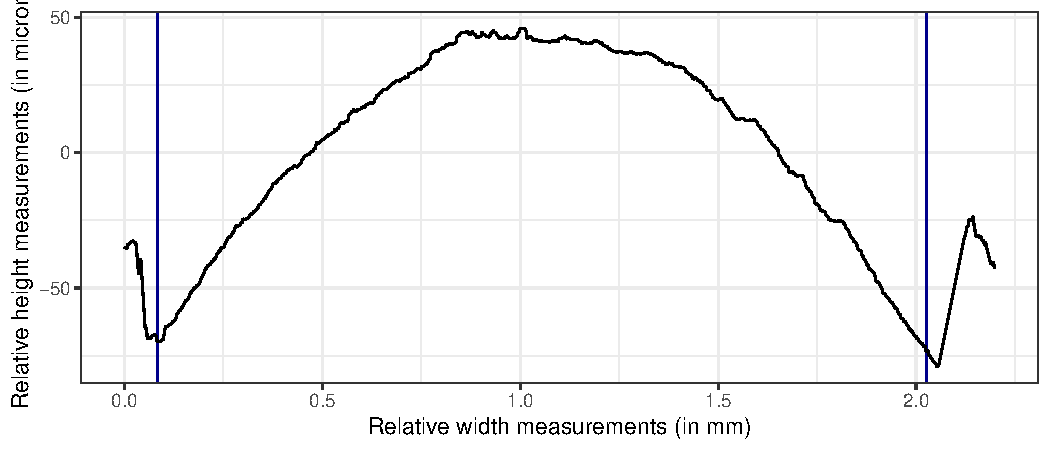
\includegraphics[width=\maxwidth]{figure/r_crosscut-motivation-1} 

}

\caption[Profile of a land engraved area (LEA), left and right groove locations are marked as vertical lines]{Profile of a land engraved area (LEA), left and right groove locations are marked as vertical lines.}\label{fig:r crosscut-motivation}
\end{figure}


\end{knitrout}

% \begin{figure}[ht!]
%   \centering
%   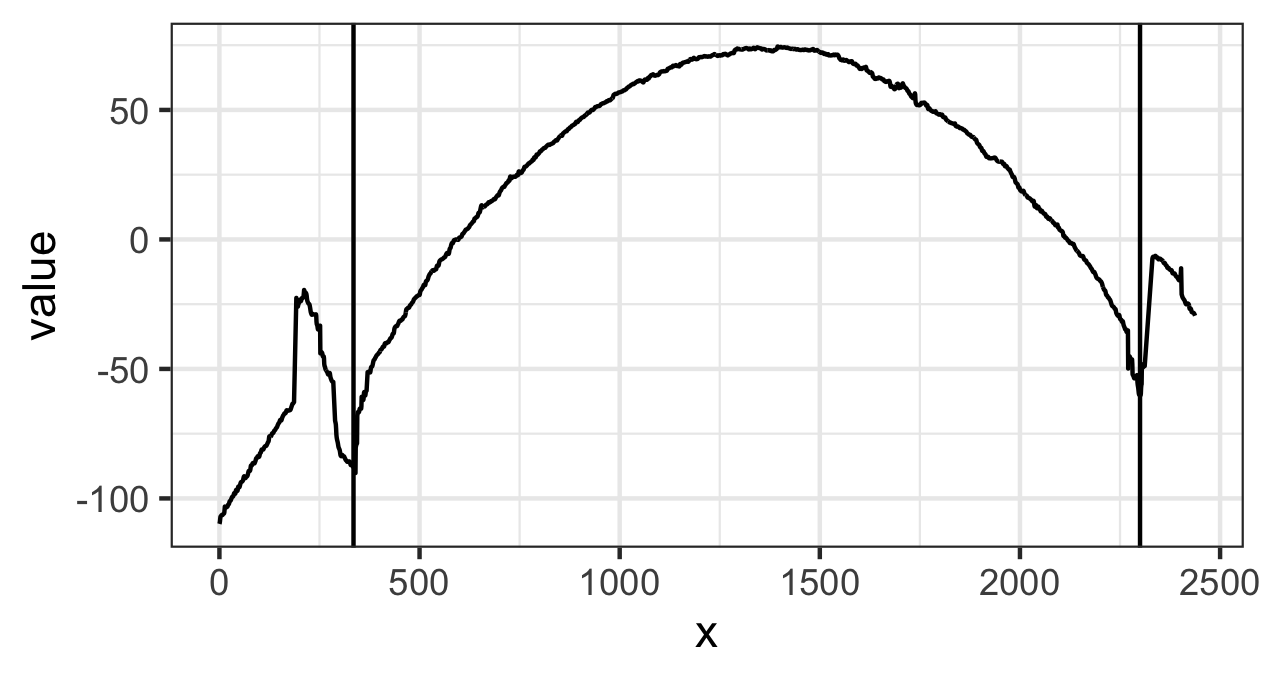
\includegraphics{../images/crosscut-motivating-image.png}
%   \caption{A single crosscut from the Hamby 44 Bullet Set, Barrel 7, Bullet 1, Land 3}
%   \label{fig:crosscut-motivation}
% \end{figure}

The predominant feature of this crosscut is the curvature of the barrel as well as two deep trenches next to two peaks which represent the beginning of the shoulders of the bullet land. To extract a signature from this data, the curvature of the bullet structure must be removed, leaving behind clear indications of striae. To accomplish this task, \cite{hare2017} fit a loess regression to the data. The residuals of this regression are then considered to be the signature of the particular bullet land in question. Due to the high variability in height of the bullet grooves or shoulder area of the bullet land, inclusion of these regions would significantly decrease the quality of the loess regression estimate of the bullet curvature since these regions are highly influential. 
\newpage

\begin{figure}[ht!]
\begin{subfigure}{.5\textwidth}
  \centering
  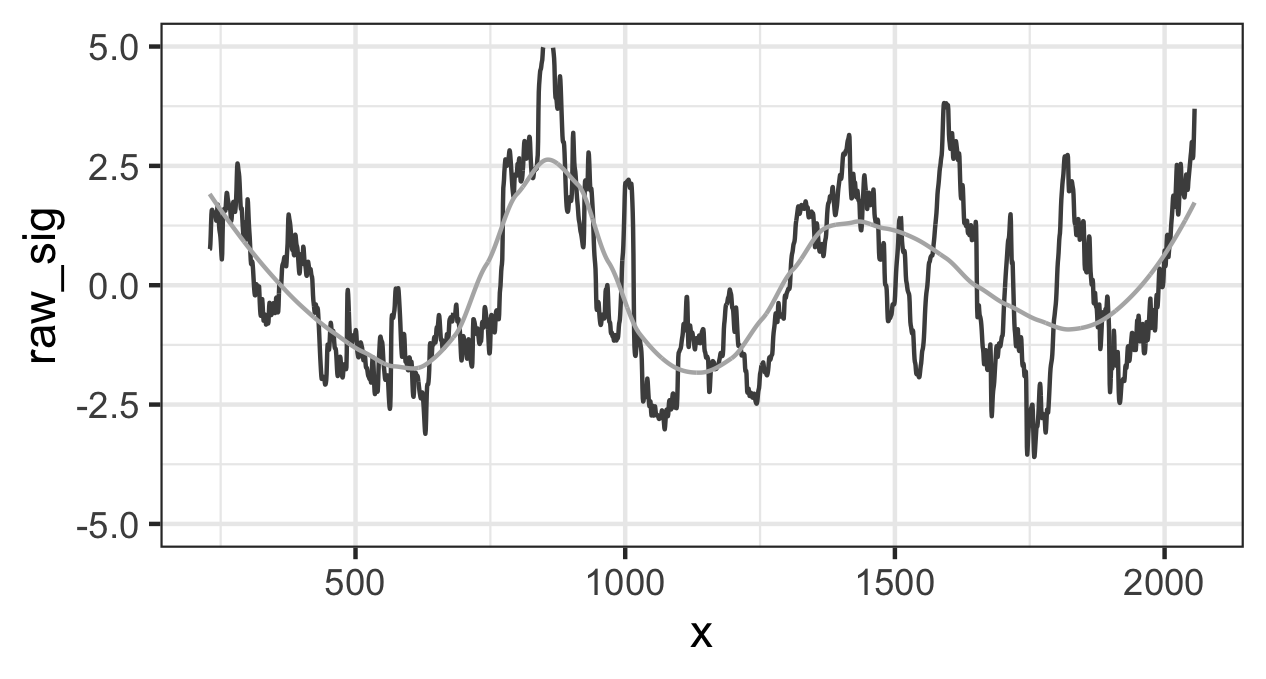
\includegraphics{../images/signal-motivating-example-good-grooves.png}
  \caption{A signature extracted from the Hamby 44 set barrel 7, bullet 1, land 3 with properly removed grooves}
\end{subfigure}
\begin{subfigure}{.5\textwidth}
  \centering
  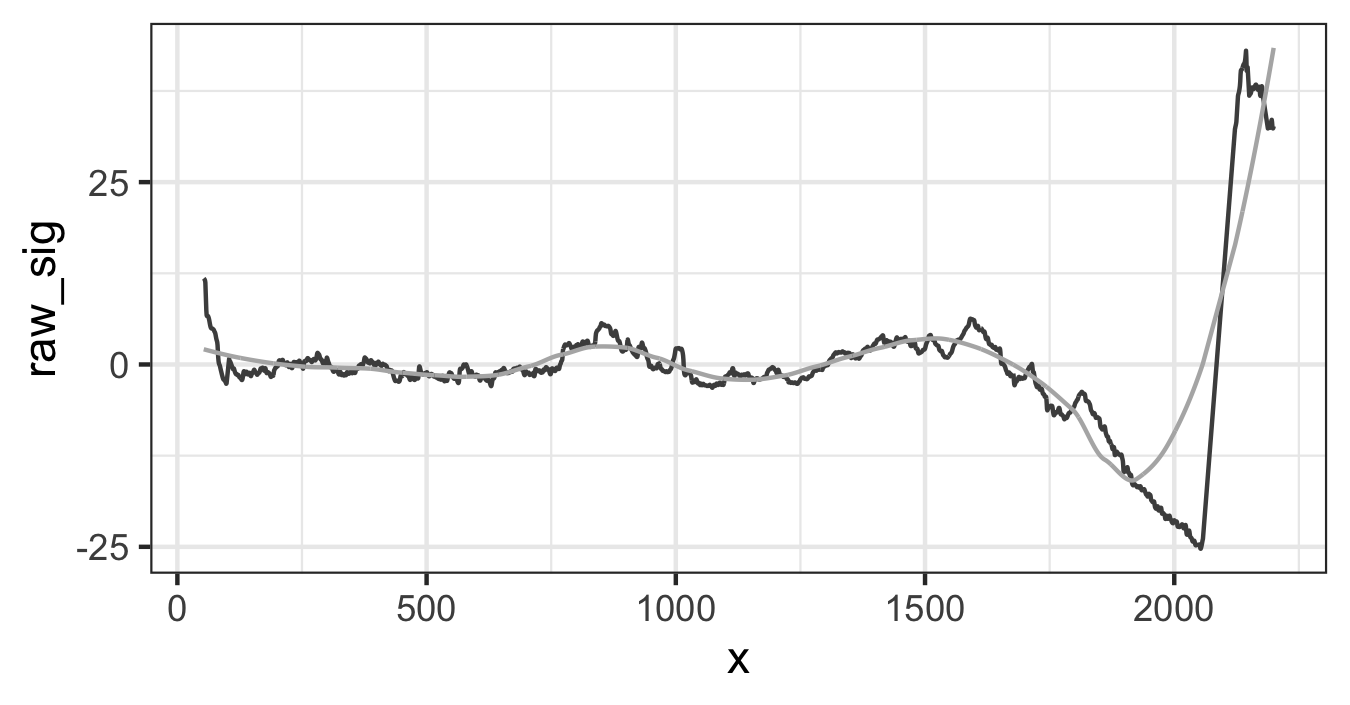
\includegraphics{../images/signal-motivating-example-bad-grooves.png}
  \caption{A signature extracted from the Hamby 44 set barrel 7, bullet 1, land 3 with improperly removed grooves}
\end{subfigure}
    \label{fig:sig-comparison}
\end{figure}

In figure \ref{fig:sig-comparison} we see a comparison between two signatures one where the grooves are properly identified and one where the grooves are improperly identified. When the right-hand groove is included the residuals are dominated by the bullet groove and the striae are no longer as pronounced. So accurately identifying the bullet grooves is supremely important for bullet identification. We propose a new method for identifying bullet grooves that utilizes an image analysis technique known as the Hough transform to identify prominent features of the bullet land. 

\subsection{Background}





\subsection{Brief Overview of Hough Transforms}

  Data for this project comes from two primary sources, Hamby 44  and Phoenix (MORE INFORMATION NEEDED). Data is stored in the form of scans called "x3p"(XML 3-D Surface Profile) and comes from high resolution 3-dimensional microscopy. Each scan consists of height measurements collected over a x-y grid, creating an image similar to a grey-scale image. To read-in and manipulate the x3p files we utilize the package `x3ptools` to orient or transform the scans as needed for image processing. When we are performing our Hough algorithm, we do not use the actual x3p-file we transform the data into a two-dimensional image. In the two-dimensional representations of bullet images, the y-axis is inverted from the standard x-y plane. A reason for this is that the images are processed in \textbf{C++} which stores images, known as ``CImgs''(Cool Images) in a vector format where the first pixel in the vector corresponds to the upper left-hand pixel of the image located at (0,0). Pixels are then ordered from left to right, extending from the origin to the positive x-direction and from top to bottom, from the x-axis towards the negative y-direction.

In broad terms, the Hough Transform is a feature extraction technique for detecting shapes in an image. For any given point in the (x,y)-plane of our image we can calculate a corresponding line in the feature space. Points that lie on the same line will have lines that intersect in the feature space. 
\begin{figure}[!ht]
\begin{subfigure}{.5\textwidth}
\centering
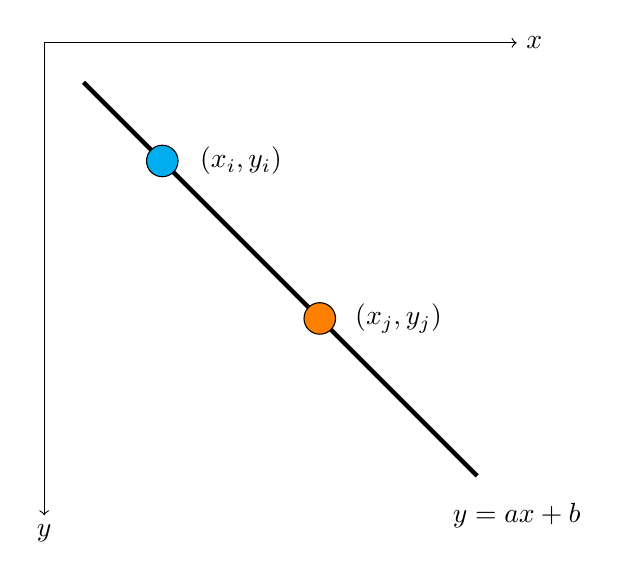
\begin{tikzpicture}
\draw [<->] (0,-6) node (yaxis) [below] {$y$} -- (0,0) -- (6,0) node (xaxis) [right] {$x$};
\draw [ultra thick] (0.5,-0.5) -- (5.5, -5.5);
\draw [fill = cyan] (1.5,-1.5) circle [radius=0.2];
\node [] at (2.5, -1.5) {($x_{i}, y_{i}$)};
\draw [fill = orange] (3.5,-3.5) circle [radius=0.2];
\node [] at (4.5, -3.5) {($x_{j}, y_{j}$)};
\node [] at (6,-6) {$y = ax + b$};
\end{tikzpicture}
\label{fig: tikz1}
\end{subfigure}
\begin{subfigure}{.5\textwidth}
\centering
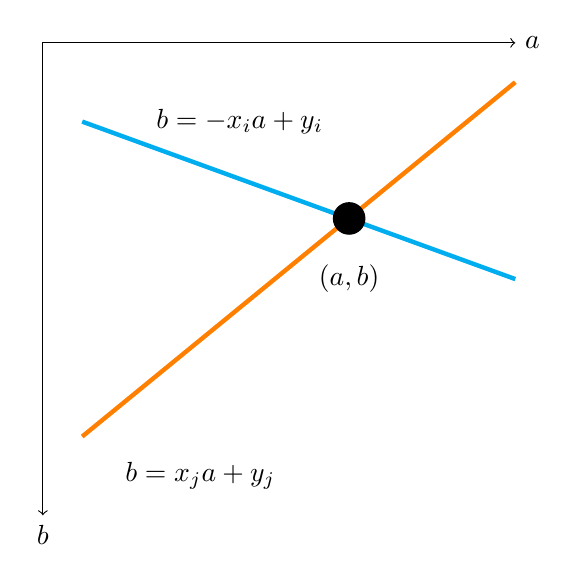
\begin{tikzpicture}
\draw [<->] (0,-6) node (yaxis) [below] {$b$} -- (0,0) -- (6,0) node (xaxis) [right] {$a$};
\draw[cyan, ultra thick] (0.5, -1) -- (6,-3);
\node [] at (2, -5.5) {$b=x_{j}a + y_{j}$};
\node [] at (2.5, -1) {$b=-x_{i}a + y_{i}$};
\draw[orange, ultra thick] (0.5, -5) -- (6,-0.5);
\draw [fill] (3.89,-2.23) circle [radius=0.2];
\node [] at (3.89, -3) {($a, b$)};
\end{tikzpicture}
\label{fig: tikz2}
\end{subfigure}
\caption{Diagram of feature space linea transformation oriented for image origin.}
\label{fig: parametrization}
\end{figure}


The point of intersection in the feature space, then corresponds to the parameters used to describe the edge in the (x,y)-plane that the two detected points lie upon. A two dimensional array called the "accumulator array" is used to keep track of features detected.  The accumulator array covers the entirety of the feature space separated into a user-specified number of bins. For each set of features detected the bin in the accumulator array associated with that set of features is incremented. So in theory, strong features should have higher values in their associated bin because there is a larger number of pixels detected that all have the same set of features in the feature space. 


\section{Methods}


In order to best identify the GEAs we first want to diminish noise in the image. This can be achieved by converting each scan into an image gradient, which signifies where there are directional changes in the color of the image. This approach unfortunately loses most of the detail of the three dimensional scans, however, it better highlights the differences between LEAs and GEAs. Once an image gradient is obtained we select only edges we consider to be "strong", meaning they have a magnitude above the 99th percentile. Our reason for not fully carrying out a Canny Edge detection algorithm before using a Hough transform is that the Canny Edge algorithm increases processing time by about 35 seconds per image and actually highlights more striae and break-off. 

\begin{figure}[!ht]
    \centering
    \begin{subfigure}{.5\textwidth}
      \centering
      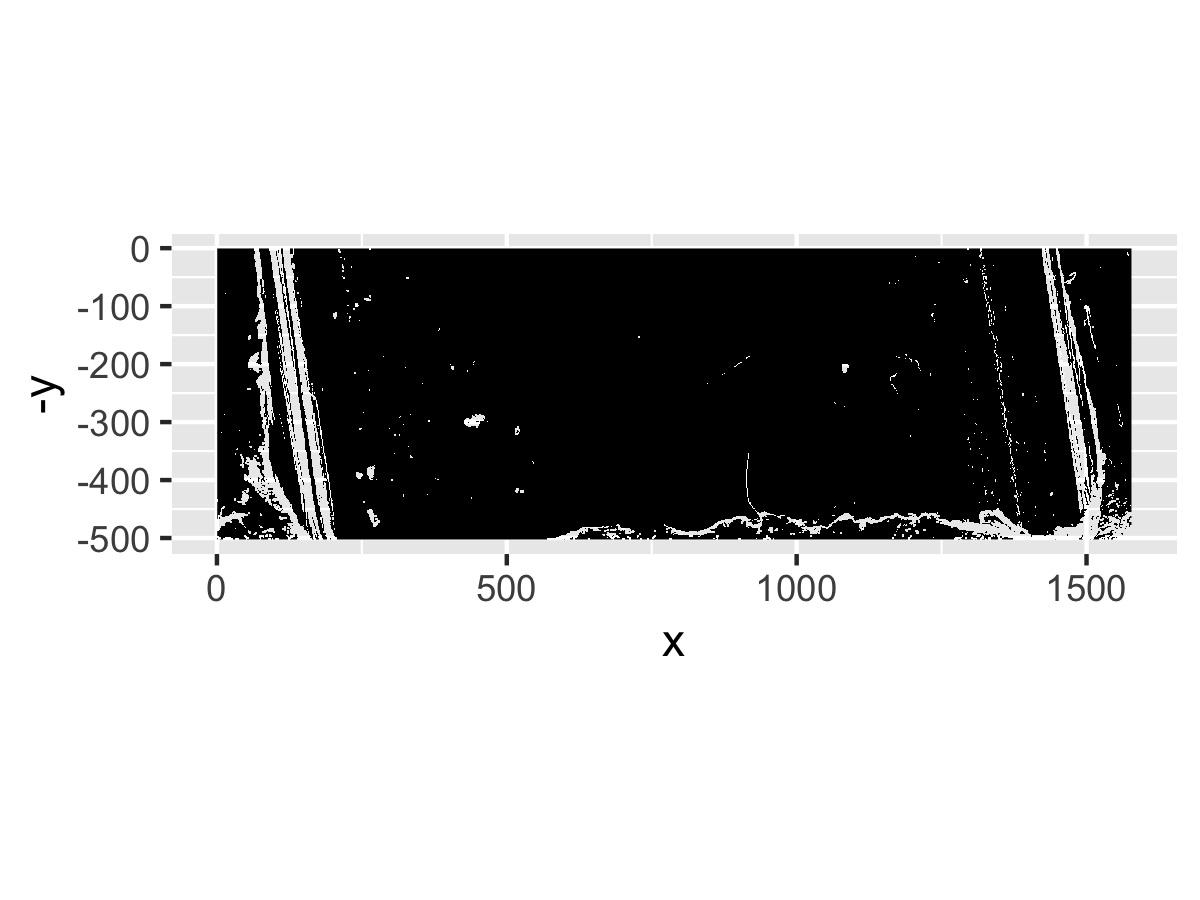
\includegraphics[width = .9\textwidth]{../images/Hamby252_Bullet1_Land3_Strong_edge.png}
      \caption{Edges with magnitudes in the 99th percentile}
      \label{fig: edge1}
      \end{subfigure}%
    \begin{subfigure}{.5\textwidth}
      \centering
      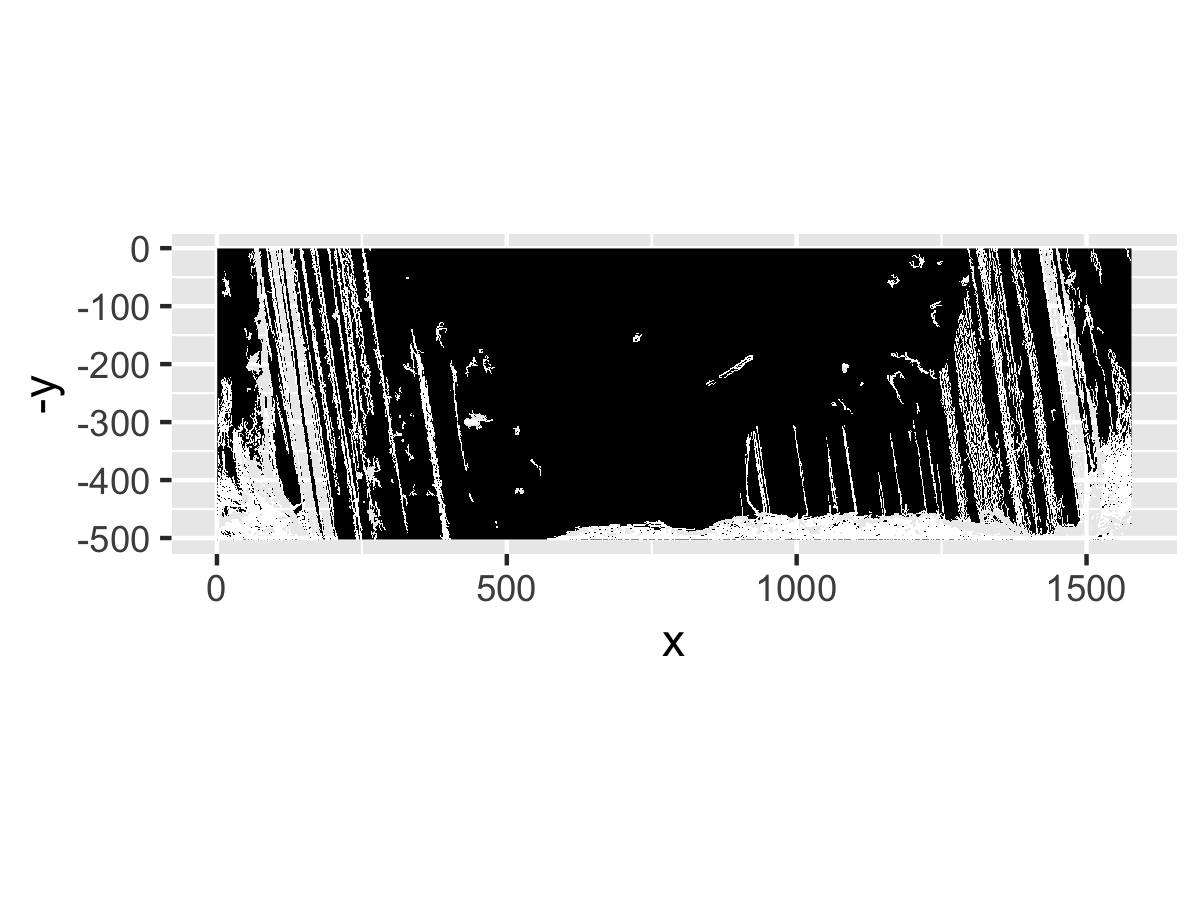
\includegraphics[width = .9\textwidth]{../images/Hamby252_Bullet1_Land3_Canny_Edge.png}
      \caption{Edges improved with Canny edge detection}
      \label{fig: edge2}
      \end{subfigure}
      \caption{Side-by-side comparison of Hamby 252 Bullet using both magnitude thresholding and Canny edge detection}
      \label{fig:canny}
\end{figure}


As shown in Figure \ref{fig:canny} the striae in the LEA are much more pronounced than in the image with only strong edges. We wish to focus on only detecting GEAs, so detecting an increased number of striae through Canny edge detection is not useful for our algorithm. Once we obtain the image gradient with only the strong edges we can then utilize our Hough transformation to obtain generally reasonable estimates of image boundaries. For the Hough transformation we utilize the function `` \texttt{hough\char`_lines}" from the imager package with the number of bins set to 100. While changing the number of bins does not seem to effect the processing time of the Hough transform, having a larger number of bins increases the number of extraneous detected lines in the image. For example in Figure \ref{fig: hough-compare}\subref{fig: hough1} we can see that the Hough transforms with 100 bins does a perfectly adequate job of picking up the suspected grooves of the bullet. Therefore the extra detected lines in \ref{fig: hough-compare}\subref{fig: hough2} are not used in our analysis so we chose to limit our bin number as a result.

\begin{figure}[!ht]
    \centering
      \begin{subfigure}{.5\textwidth}
      \centering
      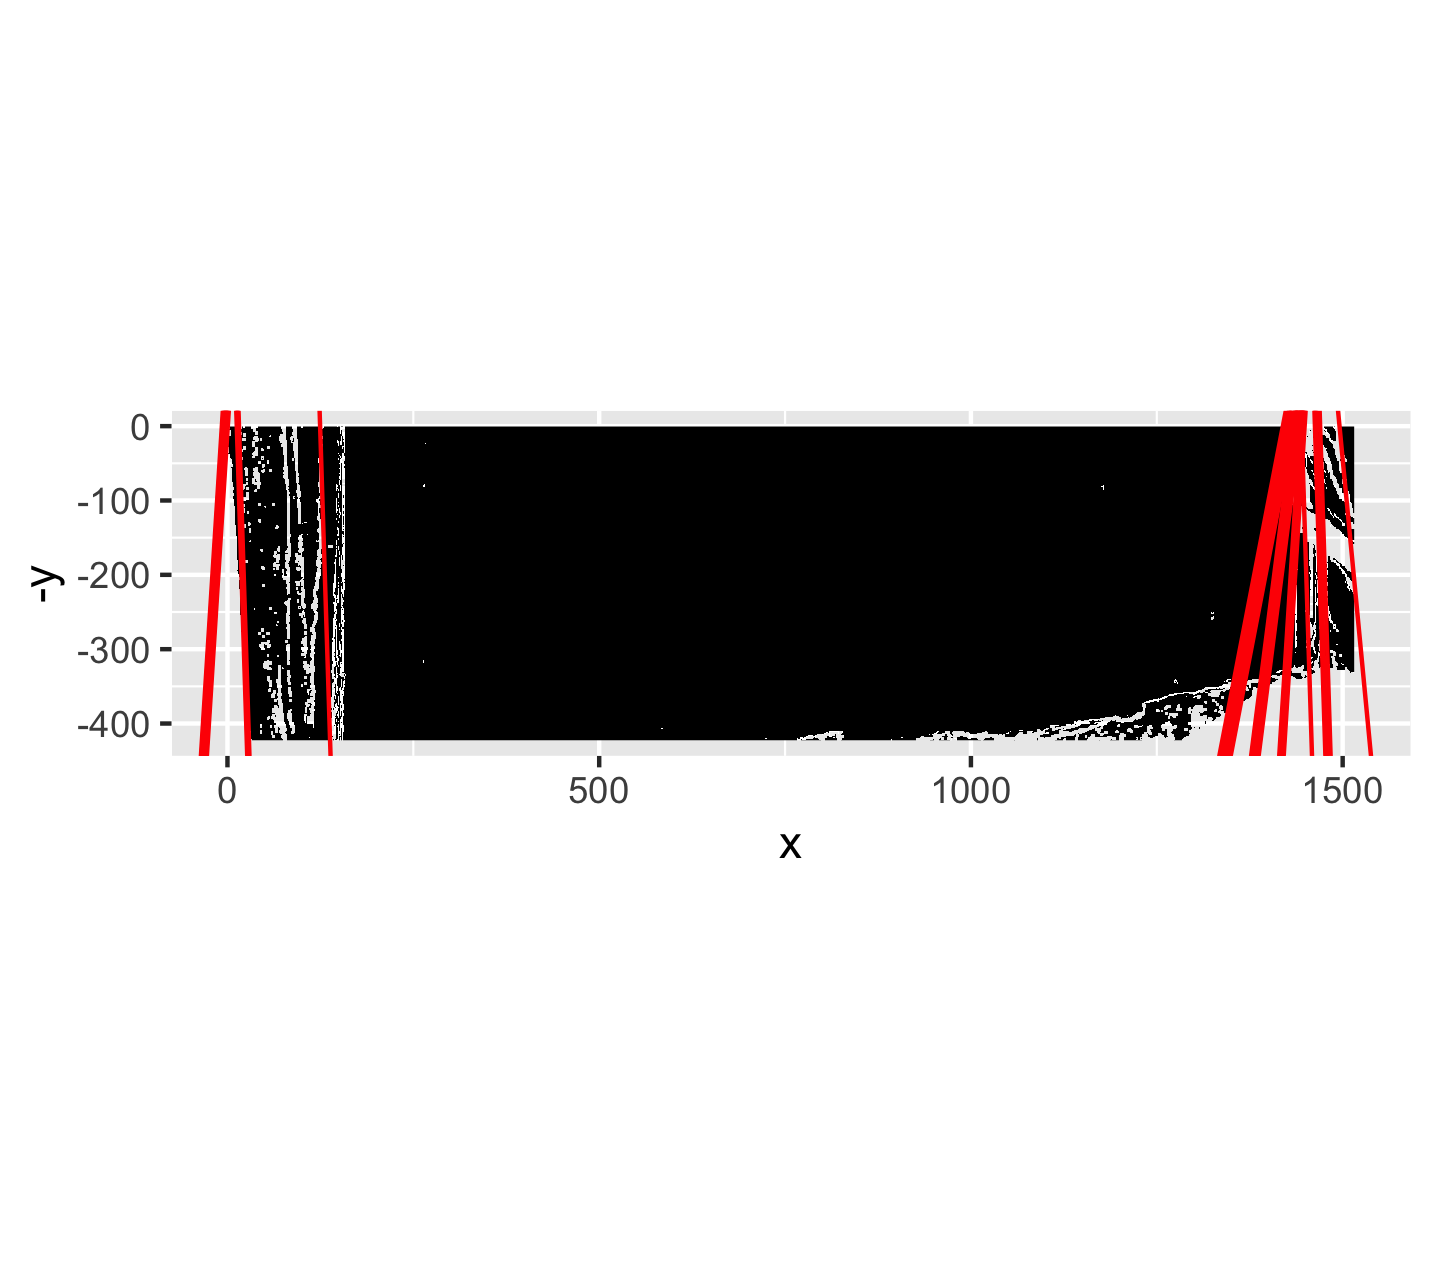
\includegraphics[width = .9\textwidth]{../images/Houston_BarrelF_Bullet1_Hough_Bin100}
      \caption{Hough Transform with 100 bins}
      \label{fig: hough1}
      \end{subfigure}%
    \begin{subfigure}{.5\textwidth}
      \centering
      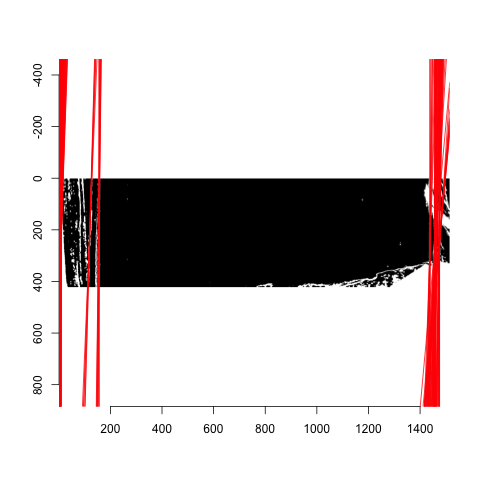
\includegraphics[width = .9\textwidth]{../images/Houston_BarrelF_Bullet1_Hough_Bin900}
      \caption{Hough Transform with 900 bins}
      \label{fig: hough2}
      \end{subfigure}
      \caption{Side-by-side comparison of Houston Barrel F Land 1 Hough Transformation. Hough lines are filtered by having scores in the 99.9th percentile, and having central angles less than $\frac{\pi}{16}$.}
      \label{fig: hough-compare}
\end{figure}

We make the assumption that scans are oriented properly and as such, most Hough lines that correlate to the GEAs will be roughly vertical with some deviations in angle based on scanning technique. It is worth noting that the original output of the `` \texttt{hough\char`_lines}" functions have angles ranging from 0 to $2\pi$. So to make selecting lines from our desired range, easier we chose to transform any angle greater than $\pi$, to instead be from 0 to $-\pi$ by subtracting $2\pi$ from the original theta angle. Therefore we select only the Hough lines that have theta angles from the positive x-axis less than $\frac{\pi}{16}$ and greater than $\frac{-\pi}{16}$. The parametrization produced by `` \texttt{hough\char`_lines}" is of the form:

\begin{center}
$\rho = x \ cos(\theta) \ + \ y \ sin(\theta)$
\end{center}

Where $\rho$ represents the length of the normalized orthogonal vector between the detected line and the origin of the image, and $\theta$ is the angle between the positive x-axis and the normalized vector. In Figure \ref{fig: parametrization} we see an example of how Hough transforms parametrize a line. In this figure, the orange line represents an example of a detected Hough line. The teal line connecting the origin to the orthogonal bisector of our detected Hough line represents the vector denoted $\rho$ in our above equation. Similarly the teal arc below represents the angle, $\theta$, which is the difference between the top of the image and the orthogonal bisector. 

\begin{figure}[ht!]
  \centering
  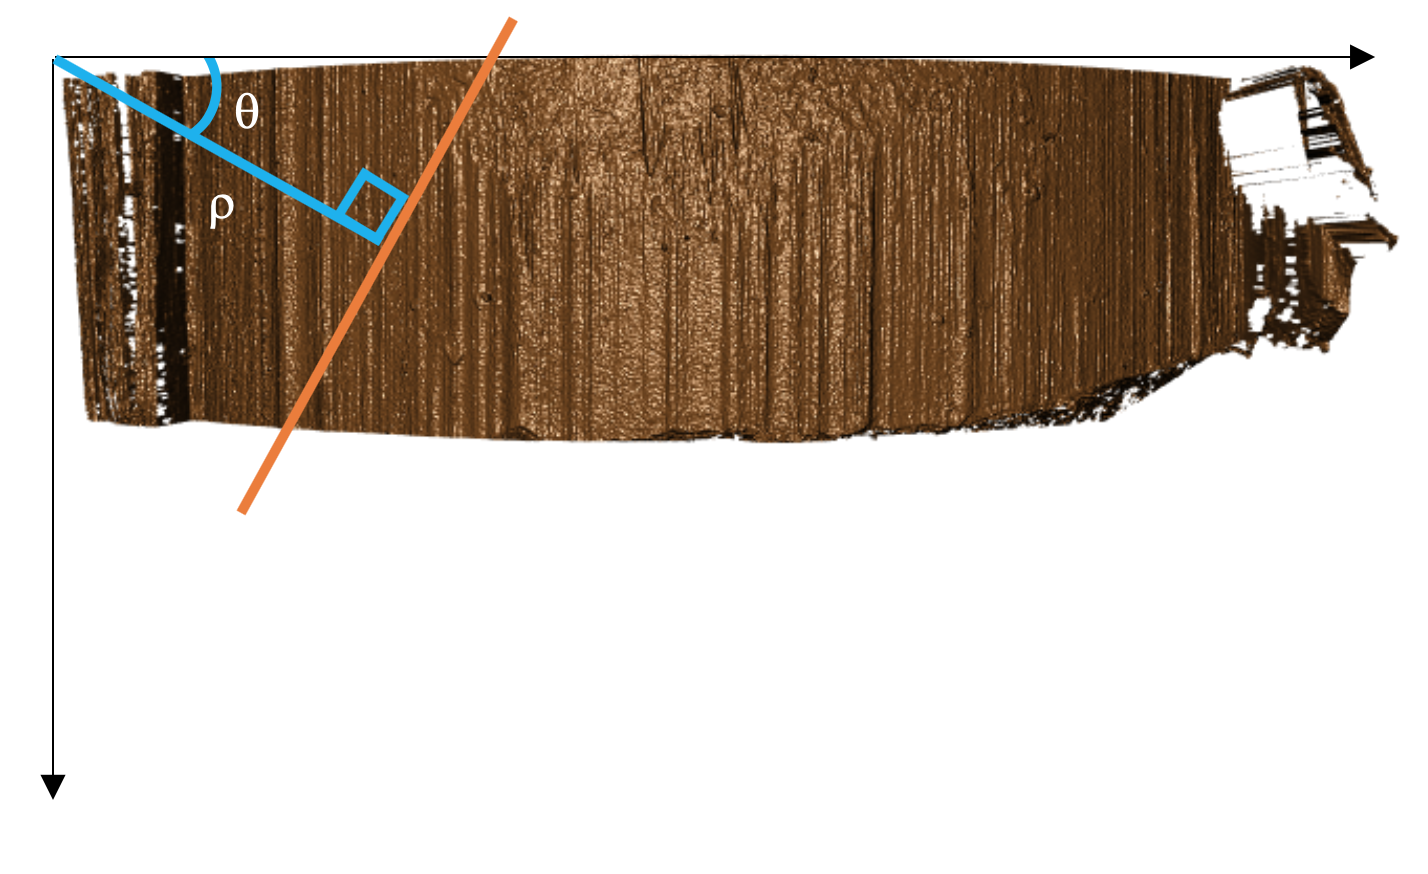
\includegraphics{../images/hessian-example.png}
  \caption{Example of Hessian Normal Form parametrization overlaid a bullet scan}
  \label{fig: parametrization}
\end{figure}

We note that when $\theta$ is equal to 0, the x-intercept is given by $\rho$ however when $\theta$ is not 0 we utilize the above equation to find that the x-intercept is equivalent to $\frac{\rho}{\cos(\theta)}$.  We utilize this calculation to find where the estimated Hough line intersects the top and bottom of the bullet land. The top is the x-intercept calculated previously, however to calculate the bottom intersection of the bullet land we utilize some geometric properties. We can draw a perpendicular line from the x-intercept at the top of the land to the bottom of the land creating a right triangle as shown below in \ref{fig: calcxbottom}. Since both the angle between the orthogonal bisector labeled $\rho$ and the new triangle created from the x-intercept to the bottom of the land are both right triangles, we know that the angle at the top of the newly formed triangle is equivalent to $\theta$. Since the x-intercept is known, we can use an elementary geometry technique to calculate the distance labeled $\delta$ in the diagram below. Since $\tan(\theta)$ is equivalent to the proportion of the length of the ``opposite" side over the ``adjacent" side of the right triangle, we know that $\delta = \tan(\theta)*\text{height}$. So the index of the bottom intersection of the bullet land is equivalent to top-intersection - $\delta$. 

\begin{figure}[ht!]
  \centering
  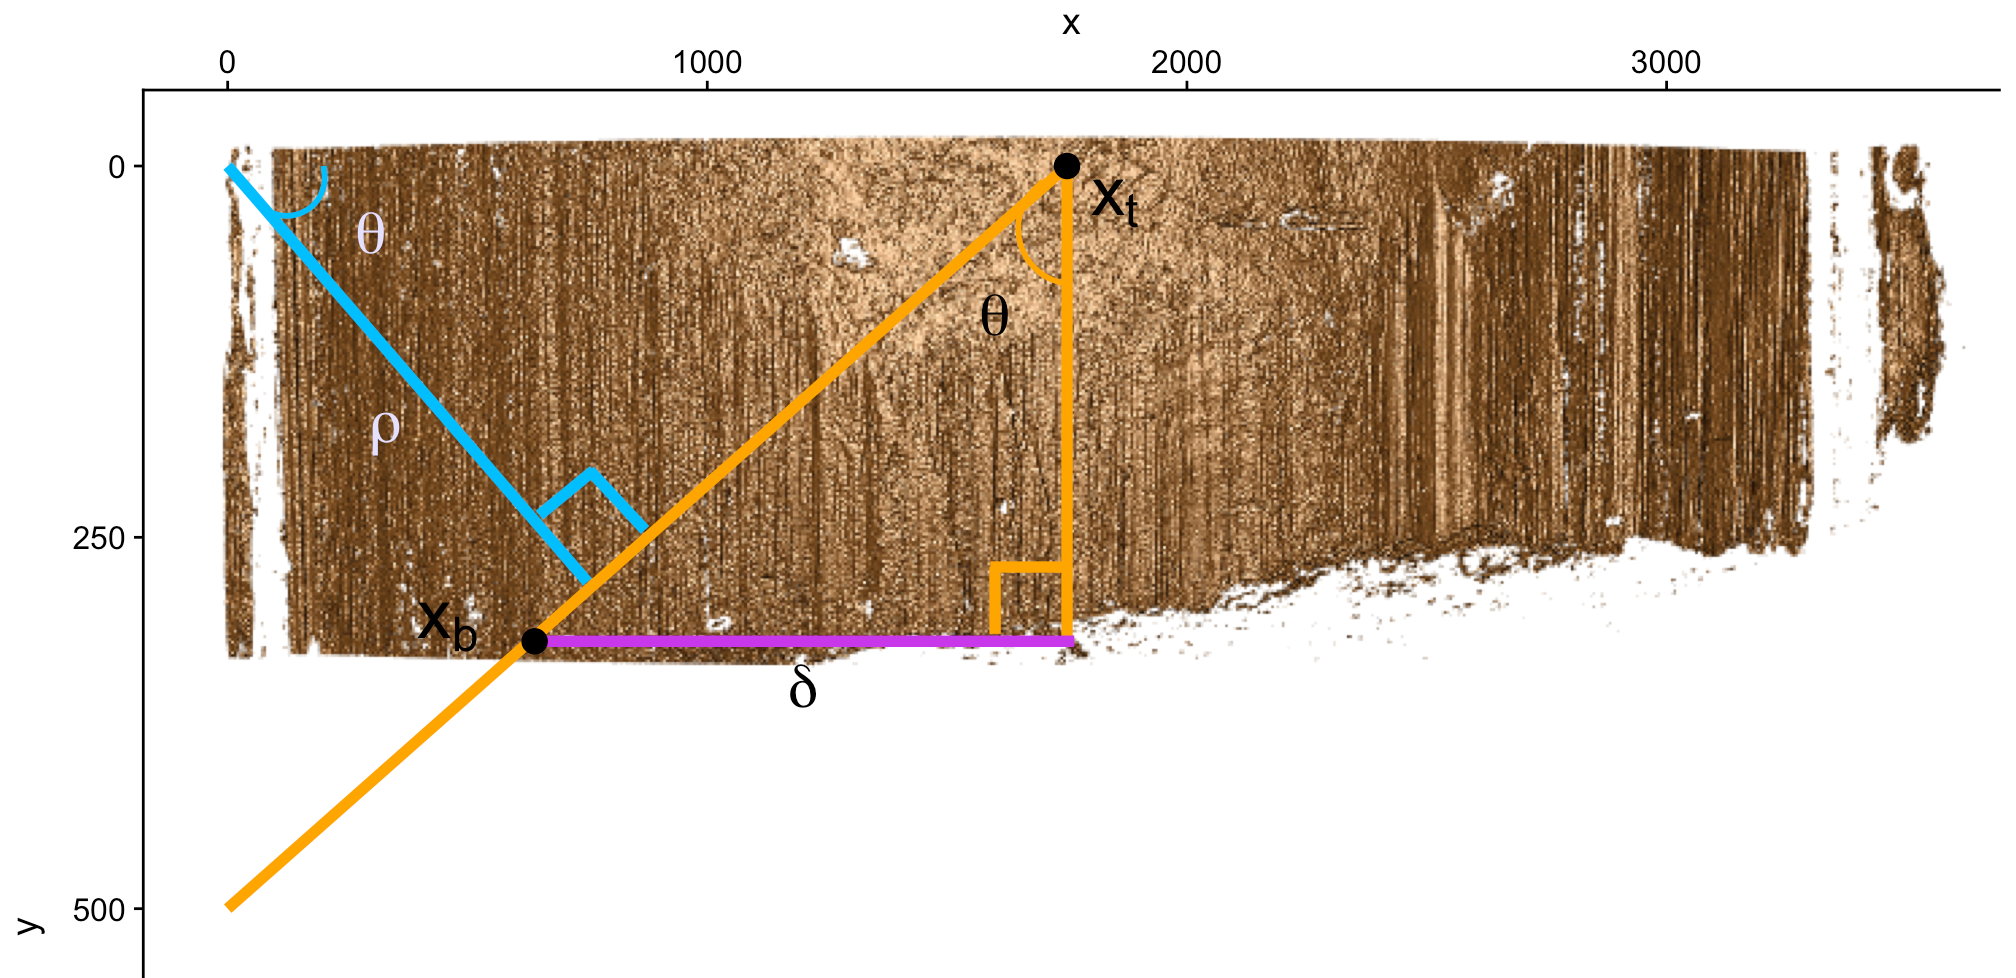
\includegraphics{../images/calc-xbottom.png}
  \caption{Demonstration of calculation of bottom intercept of a bullet land using SOH-CAH-TOA}
  \label{fig: calcxbottom}
\end{figure}

The utility for calculating the top and bottom intercept of our bullet land is that it allows us to calculate the slope of each Hough line with respect to the y-direction. 
\begin{center}
\text{Slope \ with \ respect \ to \ y} = $\frac{(\text{x-intercept of the top} - \text{x-intercept of the bottom})}{\text{height of the bullet land}}$
\end{center}

Traditionally slope with respect to the x-direction is chosen for describing the equation of a line, however, because we are primarily interested in vertical lines the slope with respect to the x-direction tends to infinity. This is undesirable because our end goal is to be able to identify the location of a bullet groove at a particular location on the y-axis, a crosscut. To identify the x-location of the groove for a given crosscut of our bullet scans, we want to input the y-location of the crosscut to our linear equation estimate of the groove and solve for x. So a slope of infinity makes this process hard to automate when we can eliminate this problem by simply having a slope in the y-direction. 

As discussed before, the Hough transform outputs a score that corresponds to the number of pixels detected on a line that can give us an indication of the strength of the feature detected. Theoretically, we would expect the strongest lines in our image to be the grooves on either side of the bullet land. So the problem arises of how best to select strong edges. Rather than simply filter scores on some arbitrary threshold, we normalize the Hough scores by the largest possible score that could be achieved for each set of features detected. The reason for this is that longer lines will have a larger Hough score simply by virtue of having a larger number of possible detectable pixels. So if we want to compare the strength of various lines, regardless of line length, we need to normalize each score associated with each line detected.  

\begin{figure}[ht!]
  \centering
  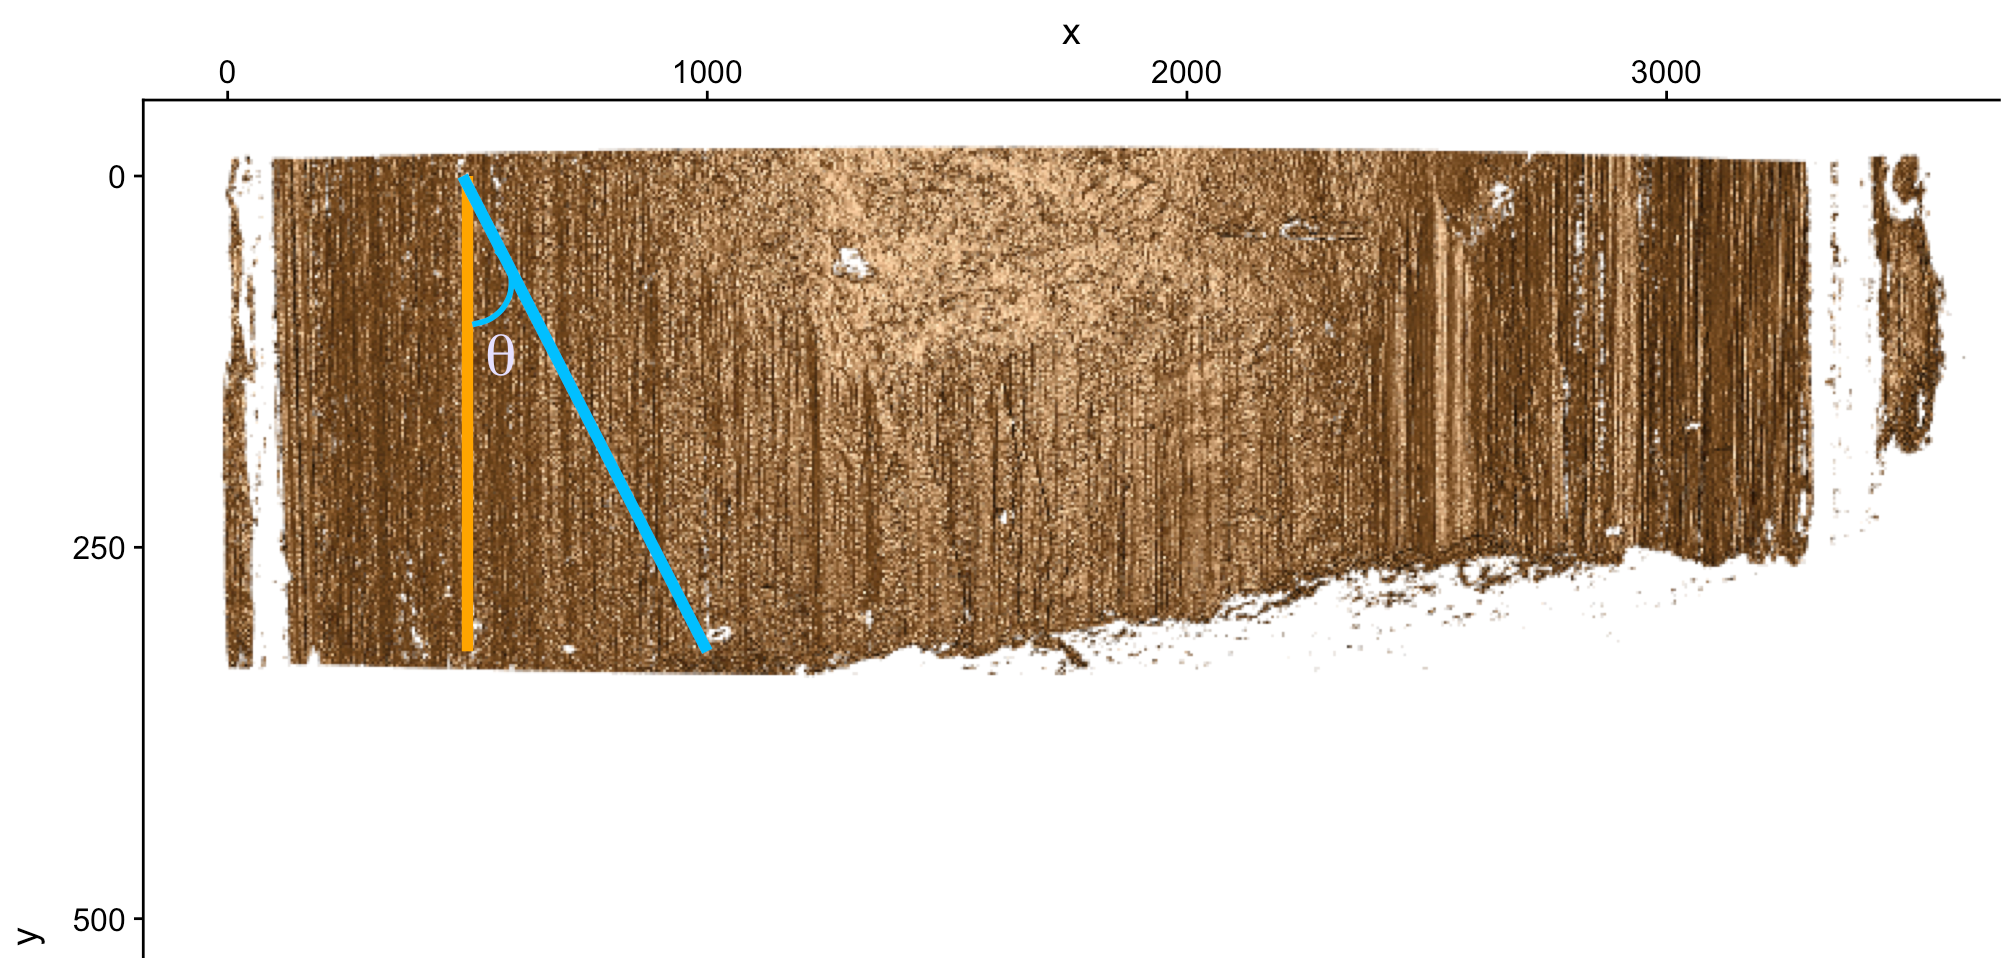
\includegraphics{../images/calc-theoretical-max.png}
  \caption{Demonstration of calculation of theoretical maximum Hough score using SOH-CAH-TOA}
  \label{fig:calcmaxscore}
\end{figure}


We calculate the largest possible theoretical score by dividing the height of the image by $\cos(\theta)$. This should in theory give us the total possible pixels that the Hough transform could have detected in our image by exploiting geometric properties of the right triangle shown in figure \ref{fig:calcmaxscore}. Then for each unique set of features that describe a line that the Hough transform detects we divide the score associated with these features by the theoretical maximum score, yielding the normalized score. 
\begin{figure}[ht!]
  \centering
  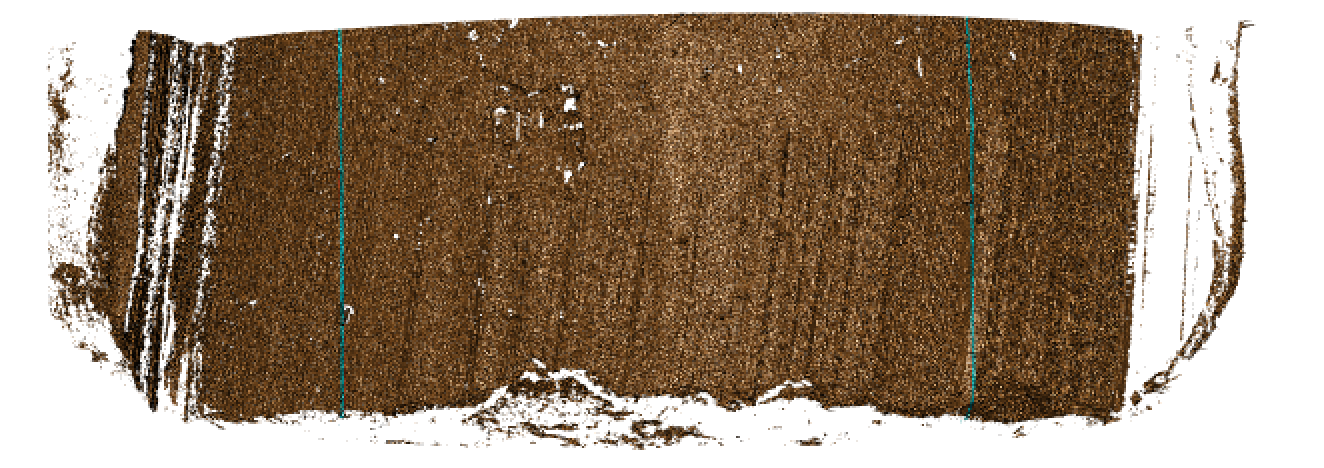
\includegraphics{../images/phnx-1-m2-b1-l1-middle-fifty-demo.png}
  \caption{Middle fifty percent of the bullet land marked by two cyan coloured vertical lines imposed over the Phoenix set Gun 1-M2 Bullet 1 Land 1 scan}
  \label{fig:middlefifty}
\end{figure}

To further specify the best candidates for the bullet land grooves, we rely on the heuristic that most of the middle 50\% of the bullet will be occupied by striae. Therefore, we can eliminate any strong lines detected within this region. An example of the middle fifty percent of a bullet land can be seen in figure \ref{fig:middlefifty} where the middle fifty percent of the bullet land is bordered by cyan colored vertical lines. We note that the grooves are well away from this middle fifty percent region, making this a suitable heuristic. We then select the highest normalized score of the lines detected outside of the middle fifty percent of the bullet land. We claim then that this is our detected bullet groove. If on the off chance that the strongest feature detected is within the middle 50\% area of the bullet land, then the grooves are set to be the borders of the middle 50\% area. 

Once features are chosen to describe both the left and right hand grooves of the bullet land the `get\_grooves\_hough` function translates these features into two equations for lines. It is worthwhile to note at this point that our calculations have been in terms of pixels detected in an image rather than the microns of the bullet scan. So we must transform our equations of lines from being in terms of pixels to microns. This is accomplished inside the `get\_grooves\_hough` function by the helper function `pix\_to\_micron` which subtracts one from the pixel location (since pixels start indexed at one and microns start indexed at zero), then multiplies that pixel location by the resolution of the x3p-scan. Because we are interested in the slope with respect to the y-direction we calculate our linear equations as follows:

\begin{center}
  $\text{Groove Estimate} = \text{Bottom x-intercept in microns} + \text{slope}*y_{i} - \text{adjust}$
\end{center}

 Unlike other methods available in the `GrooveFinder` package, the `get\_grooves\_hough` function does not provide a groove estimate at an optimized crosscut. The output of the  `get\_grooves\_hough` function are a set of two functions that correspond to the left and right-hand grooves. So to produce an actual estimate of our groove location we need to input a y-location into our two functions. For a single point-estimate we can input the y-location of a single crosscut using the `x3p\_optimize\_crosscut` function from the `bulletxtrctr` package. However to visualize our groove estimates across the entire bullet land we have created a helper function called `get\_mask\_hough` that creates a colored mask over our bullet land of our groove estimates as shown in \ref{fig:get-mask-hough-example-one}. 
 
\begin{figure}[ht!]
  \centering
  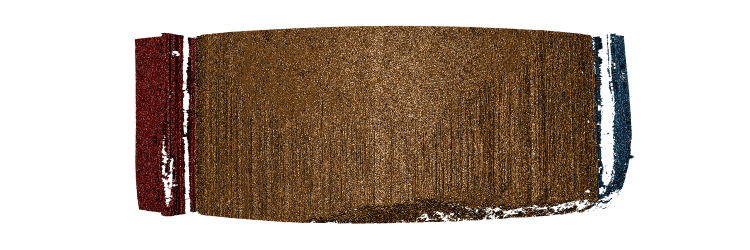
\includegraphics{../images/phoenix-gun-1-l5-b1-l1-groove-estimation-example-1.png}
  \caption{Hough groove estimate visualized over whole of bullet land for the Phoenix set gun 1-L5 bullet one land one with adjust set to 30.}
  \label{fig:get-mask-hough-example-one}
\end{figure}


\section{Results}



\bibliography{summat} % Tells it where your list of references is.
\bibliographystyle{plainnat} 

\end{document}
